\chapter{振子波函數、自旋二分之一與粒子交換}

\section{無所不在的振子}

任何具有穩定平衡位置的系統，受到偏離平衡位置的擾動時都可能振盪。它可能只有一個頻率，也可能有許多頻率。例如，小提琴弦有基音模態和更高次的諧波。撥動琴弦會激發這些模態的某種組合。

這裡更重要的例子是場。電磁場的平衡態是真空：沒有電場、沒有磁場，也沒有電磁振盪。將輻射導入腔體或波導後，場可以在其允許的模態中振盪，每個模態都有自己的頻率。在量子理論中，這些模態描述的是光子的集合。

同樣的想法也適用於晶體。若把每個原子都想成獨立的振子，便會產生誤解。原子彼此施力，因此一個原子的位移會影響鄰近原子，波也會在晶體中傳播。這種耦合運動的正規模態是諧振子，其量子稱為聲子。光子和聲子是不同的物理對象，但兩者都可歸結為相同的振子代數。

\section{振子代數}

討論振子時，令質量和約化普朗克常數都等於一：
\[
m=1,\qquad \hbar=1.
\]
哈密頓量為
\begin{equation}
H=\frac{p^{2}}{2}+\frac{\omega^{2}x^{2}}{2}.
\end{equation}
參數\(\omega\)決定勢能的曲率，也就是振盪頻率。

定義升算符和降算符如下：
\begin{equation}
A_{\pm}=\frac{p\pm i\omega x}{\sqrt{2\omega}}.
\end{equation}
其正規化方式使得
\begin{equation}
[A_{-},A_{+}]=1.
\end{equation}
數算符為
\begin{equation}
N=A_{+}A_{-}.
\end{equation}
這些方程合起來表示，\(A_{+}\)會使\(N\)的本徵值增加一，而\(A_{-}\)會使之減少一。因此，能譜為
\begin{equation}
n=0,1,2,3,\ldots .
\end{equation}

將兩個階梯算符相乘，也可看出經典能量的量子修正：
\begin{align}
N
&=\frac{1}{2\omega}(p+i\omega x)(p-i\omega x)\\
&=\frac{1}{2\omega}\left(p^{2}+\omega^{2}x^{2}
 +i\omega[x,p]\right)\\
&=\frac{1}{2\omega}\left(p^{2}+\omega^{2}x^{2}-\omega\right),
\end{align}
其中\([x,p]=i\)。因此，
\begin{equation}
H=\omega\left(N+\frac12\right).
\end{equation}
若附加常數與問題無關，使用平移後的哈密頓量會較方便：
\begin{equation}
H_{\mathrm{shifted}}=H-\frac{\omega}{2}=\omega N.
\end{equation}
項\(\omega/2\)是振子的零點能，也就是基態能量。對場模態而言，相應的項稱為真空能。它反映了不確定性原理：沒有任何態能讓\(x\)和\(p\)同時精確等於零，因此\(H\)中的兩個正二次項，其期望值不可能同時為零。

\begin{classroomqa}
\lecturetimestamp{00:09:46}
\audiencequestion{為什麼數算符的譜包含零？}
\lecturerresponse{可以藉由明確構造基態波函數來證明。這個構造會找出一個滿足\(N=0\)的態。}
\end{classroomqa}

要開始這個構造，可以用位置波函數取代態向量。能量本徵態變成
\[
\psi_{0}(x),\ \psi_{1}(x),\ \psi_{2}(x),\ldots,
\]
而基本算符的作用方式為
\begin{equation}
X\longmapsto x,\qquad
P\longmapsto -i\frac{d}{dx}.
\end{equation}
恢復\(\hbar\)後，第二個替換應為
\(P\mapsto-i\hbar\,d/dx\)。

在求解\(\psi_{0}\)之前，這個問題有個更快的抽象解答。在可正規化振子本徵態構成的離散階梯上，\(N=A_{+}A_{-}\)是非負的，因此不可能以單位步長無限地反覆降低。在階梯底端---其可正規化波函數將於下文構造---處，必定有一個態，記為\(\lvert0\rangle\)，滿足
\begin{equation}
A_{-}\lvert0\rangle=\mathbf 0.
\end{equation}
否則，\(A_{-}\lvert0\rangle\)會是再低一階的另一個態。立即可得
\begin{equation}
N\lvert0\rangle
=A_{+}A_{-}\lvert0\rangle
=\mathbf 0
=0\,\lvert0\rangle.
\end{equation}
因此，底端態的數本徵值為零。

\begin{classroomqa}
\lecturetimestamp{00:14:57}
\audiencequestion{若本徵值是零，等式右側是否應該是零本徵向量？}
\lecturerresponse{右矢\(\lvert0\rangle\)是正規化的非零向量，其標記為零。在\(N\lvert0\rangle=0\,\lvert0\rangle\)中，等式右側是零向量。基態右矢和零向量是不同的對象。}
\end{classroomqa}

\section{薛丁格Schr\"odinger方程與物理解}

現在回到位置表象。不含時的Schr\"odinger方程為
\begin{equation}
\left[
-\frac12\frac{d^{2}}{dx^{2}}
+\frac12\omega^{2}x^{2}
\right]\psi(x)=E\psi(x).
\end{equation}
作為一個二階微分方程，它對任意\(E\)值都有形式解。但其中大多數形式解都不是物理上可接受的振子態；它們在\(\lvert x\rvert\)很大時會指數增長，使其範數發散。

束縛態的波函數必須平方可積：
\begin{equation}
\int_{-\infty}^{\infty}\psi^{*}(x)\psi(x)\,dx<\infty.
\end{equation}
如此一來，就可以將波函數正規化，使積分等於一。只有特定的能量值才會產生這類解。無限直線上的位置態和動量態在這方面是例外；至於指數增長的振子解，則直接排除於態空間之外。

\section{高斯基態}

這個二階方程可以求解，但利用階梯代數可得到更簡單的一階方程：
\begin{equation}
A_{-}\psi_{0}(x)=0.
\end{equation}
等式右側為零時，\(A_{-}\)的整體因子不影響結果，因此這等價於
\begin{equation}
(p-i\omega x)\psi_{0}(x)=0.
\end{equation}
利用\(p=-i\,d/dx\)可得
\begin{equation}
\left(\frac{d}{dx}+\omega x\right)\psi_{0}(x)=0.
\end{equation}

\begin{classroomqa}
\lecturetimestamp{00:22:32}
\audiencequestion{可以用變數分離法求解嗎？}
\lecturerresponse{只有一個自變數，沒有兩個變數可以分離。把方程寫成\(\psi_{0}'/\psi_{0}=-\omega x\)的形式，就能看出它是對數導數。這提示我們將波函數寫成指數形式。}
\end{classroomqa}

一種簡便的解法是令
\begin{equation}
\psi_{0}(x)=e^{f(x)}.
\end{equation}
於是
\[
\psi_{0}'(x)=f'(x)e^{f(x)},
\]
約去兩邊相同的指數因子後，方程化為
\begin{equation}
\frac{df}{dx}+\omega x=0.
\end{equation}

\begin{classroomqa}
\lecturetimestamp{00:26:28}
\audiencequestion{\(f(x)\)裡應該有一個負號嗎？}
\lecturerresponse{是的。由於\(df/dx=-\omega x\)，積分後會得到負的二次項。}
\end{classroomqa}

因此
\begin{equation}
f(x)=-\frac12\omega x^{2}+C,
\end{equation}
而且
\begin{equation}
\psi_{0}(x)\propto e^{-\omega x^{2}/2}.
\end{equation}
乘法正規化常數不必明確指定。關鍵在於其高斯形狀：波函數平滑、集中在原點附近，並在\(\lvert x\rvert\)很大時迅速衰減。顯然它是平方可積的。

無須將答案代回二階方程，就能求出其能量。代數已經給出
\begin{equation}
E_{0}=\frac{\omega}{2}.
\end{equation}

\section{激發態、節點與經典運動}

對基態作用升算符，即可得到第一激發態：
\begin{equation}
\psi_{1}(x)\propto A_{+}\psi_{0}(x)
\propto(p+i\omega x)e^{-\omega x^{2}/2}.
\end{equation}
基態方程給出
\[
p\psi_{0}=i\omega x\,\psi_{0}.
\]
改變階梯算符中的符號，就會把相消變成相加：
\begin{equation}
(p+i\omega x)\psi_{0}
=2i\omega x\,\psi_{0}.
\end{equation}
略去整體常數後，
\begin{equation}
\psi_{1}(x)\propto x\,e^{-\omega x^{2}/2}.
\end{equation}

這個波函數是奇函數：
\begin{equation}
\psi_{1}(-x)=-\psi_{1}(x).
\end{equation}
它的機率密度是偶函數，但在原點有一個節點：
\begin{equation}
\lvert\psi_{1}(0)\rvert^{2}=0.
\end{equation}
因此，第一激發態的機率密度在\(x=0\)有一個節點。

反覆作用\(A_{+}\)，會得到乘上相同高斯包絡的高次多項式。\footnote{講課中說明，高次多項式因子每升一階便多一個節點，對稱性則從\(00{:}34{:}25\)到\(00{:}35{:}49\)交替變化。Leonard Susskind 與 Art Friedman 在\emph{Quantum Mechanics: The Theoretical Minimum}（2014）討論振子本徵函數時，也印證了高斯函數乘上多項式的形式。}略去正規化因子後，
\begin{equation}
\psi_{n}(x)=P_{n}(x)e^{-\omega x^{2}/2}.
\end{equation}
宇稱在偶與奇之間交替，每升一階便增加一個節點。隨著\(n\)增大，波函數會延伸到離原點更遠處，並且振盪得更快。

這兩個特徵都有直接的物理意義。波函數延伸到離原點更遠處，表示勢能較大，因為勢能隨\(x^{2}\)增加。位置空間中的快速振盪則代表較大的動量。高度激發的振子更可能到達離中心較遠處；它通過中心區域時，動量較大，波函數在該處也振盪得更快。

\begin{classroomqa}
\lecturetimestamp{00:37:18}
\audiencequestion{當\(n\)變大時，諧振子會不會仍無法呈現經典行為？}
\lecturerresponse{經典運動並非由單一定態能量本徵態表示，而是出現在包含許多能階的波包中。例如，位移後的高斯波包會像經典振子一樣來回運動；而擺動幅度越大，相對不確定度就越小。}
\end{classroomqa}

從基態高斯波包開始，將它從原點平移開來。平移後的波包不再是能量本徵態，而是許多能量本徵態的疊加。在含時Schr\"odinger方程的演化下，各分量會獲得不同的相位。波包在勢能的一側和另一側之間往返，在中心附近產生快速的相位變化，到了轉折點附近則再次變得平滑。相較於波包的寬度，位移越大，運動就越接近經典情況。

\begin{classroomqa}
\lecturetimestamp{00:39:29}
\audiencequestion{第二激發態的波函數是否應該在原點為零？}
\lecturerresponse{不會。它的多項式因子不只是\(x^{2}\)，還包含一個常數項，因此波函數不一定在\(x=0\)為零。}
\end{classroomqa}

階梯論證也假設\(A_{+}\)和\(A_{-}\)在振子的平方可積函數定義域上互為厄米共軛，並滿足伴隨關係所需的邊界條件。指數增長的形式解不屬於這個定義域。

\begin{classroomqa}
\lecturetimestamp{00:40:45}
\audiencequestion{有沒有通用的方法，能判斷哪些哈密頓量可以用這些代數方法求解？}
\lecturerresponse{沒有這樣的通用規則。精確可解的例子很少。諧振子和理想的非相對論氫原子是少數能用代數方法求解的例子。}
\end{classroomqa}

\section{自旋二分之一作為角動量}

自旋是粒子本身攜帶的角動量，與其質心的軌道運動無關。靜止的粒子沒有軌道角動量\(\mathbf R\times\mathbf P\)，但仍可能有自旋。可以試著把它想像成微小的旋轉物體，也可以把自旋視為內禀的量子性質。關鍵的陳述在於數學形式：自旋的分量會隨空間旋轉而變換，並遵守角動量對易關係。

從此處起恢復\(\hbar\)。角動量分量滿足
\begin{equation}
[L_{z},L_{x}]=i\hbar L_{y},
\end{equation}
另外兩個關係可由循環置換得到。無因次的泡利矩陣為
\begin{equation}
\begin{aligned}
\sigma_{z}&=
\begin{pmatrix}
1&0\\
0&-1
\end{pmatrix},\\[0.4em]
\sigma_{x}&=
\begin{pmatrix}
0&1\\
1&0
\end{pmatrix},\\[0.4em]
\sigma_{y}&=
\begin{pmatrix}
0&-i\\
i&0
\end{pmatrix}.
\end{aligned}
\end{equation}
在這個基底中，\(\sigma_{z}\)是對角矩陣，其本徵值為\(+1\)和
\(-1\)。

\begin{classroomqa}
\lecturetimestamp{00:47:35}
\audiencequestion{\(\sigma_x\)裡有負號嗎？}
\lecturerresponse{沒有。\(\sigma_x\)的兩個非對角元素都是正的。}
\end{classroomqa}

\(00{:}49{:}35\)的板書計算從逐項相乘開始。完成矩陣乘法後可得
\begin{align}
\sigma_{z}\sigma_{x}
&=
\begin{pmatrix}
0&1\\
-1&0
\end{pmatrix}
=i\sigma_{y},\\
\sigma_{x}\sigma_{z}
&=
\begin{pmatrix}
0&-1\\
1&0
\end{pmatrix}
=-i\sigma_{y}.
\end{align}
因此
\begin{equation}
[\sigma_{z},\sigma_{x}]=2i\sigma_{y}.
\end{equation}
定義物理自旋算符時加入下式，即可消去多出的因子二。\footnote{板書計算省略了\(\hbar\)；此處將它補回，使\(S_i\)具有角動量的單位。}
\begin{equation}
S_{i}=\frac{\hbar}{2}\sigma_{i}.
\end{equation}
於是
\begin{equation}
[S_{z},S_{x}]=i\hbar S_{y},
\end{equation}
循環置換的情形也相同。因此，將\(\hbar\)因子補回後，半個泡利矩陣便構成一組角動量算符。

令\(\hbar=1\)，即可得到如下形式。\footnote{來源影格為\texttt{lecture\_04\_frame\_02.png}。}
\begin{figure}[htbp]
\centering
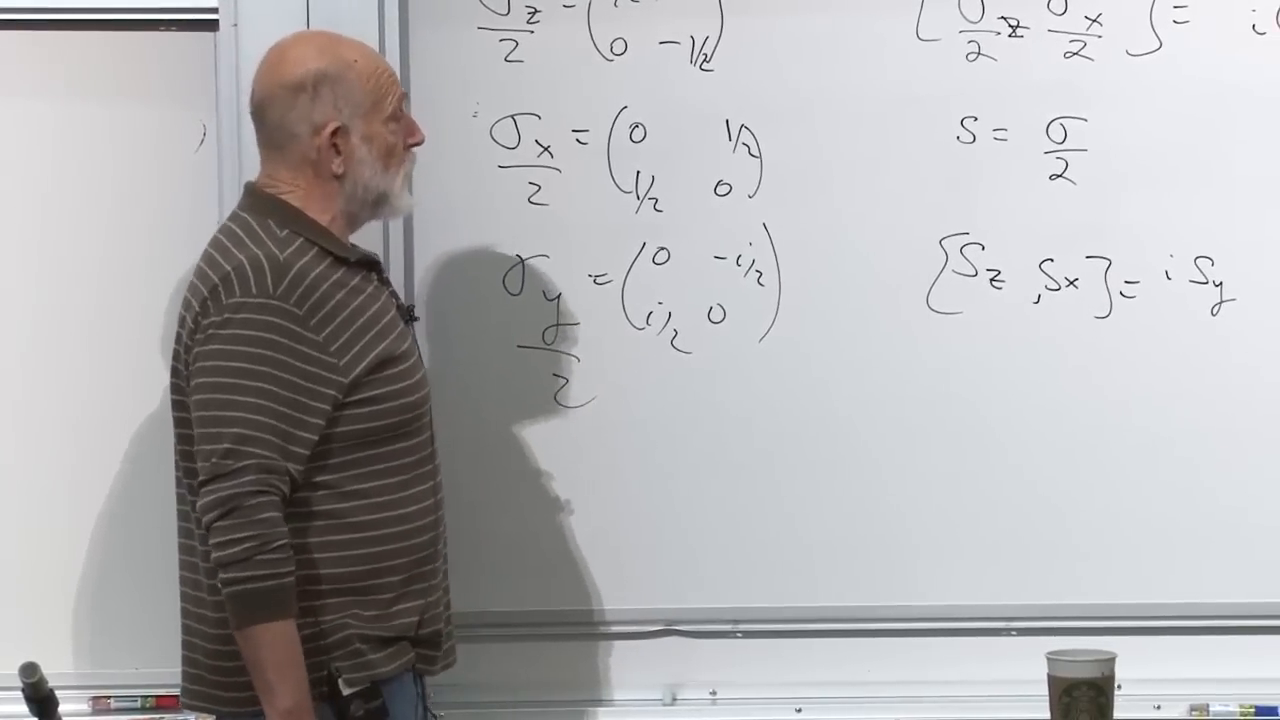
\includegraphics[width=0.9\linewidth]{lecture_04_frame_02.png}
\caption{在\(\hbar=1\)的單位制下，泡利矩陣的一半是自旋二分之一的角動量算符，並滿足\([S_z,S_x]=iS_y\)。}
\lectureframe{00:55:41}
\end{figure}

兩個\(S_z\)本徵值方程為
\begin{equation}
S_z\lvert\pm\rangle
=\pm\frac{\hbar}{2}\lvert\pm\rangle.
\end{equation}
等價地，無因次的磁量子數為
\begin{equation}
m_{s}=\pm\frac12,
\qquad
S_{z}\lvert m_{s}\rangle
=m_{s}\hbar\,\lvert m_{s}\rangle.
\end{equation}
角動量升、降算符會使\(m\)以整數步長改變，但這不表示每個階梯都必須經過零。整數多重態包含整數\(m\)值，半整數多重態則包含半整數值。自旋二分之一的階梯只有\(m_s=+1/2\)和\(m_s=-1/2\)兩個態。

這兩個態構成自旋二分之一的雙重態。電子、{\proseunicodefont μ}子、中微子和夸克都是以這類半整數自旋多重態描述的粒子。

\section{軌道角動量與自旋角動量}

現在有兩種角動量。軌道角動量描述相對於原點的運動：
\begin{equation}
\mathbf L=\mathbf R\times\mathbf P,
\end{equation}
而\(\mathbf S\)是內禀自旋。兩者的向量和就是總角動量：
\begin{equation}
\mathbf J=\mathbf L+\mathbf S.
\end{equation}

\begin{classroomqa}
\lecturetimestamp{00:56:49}
\audiencequestion{若系統的總角動量為\(\mathbf J\)，要如何判定它的自旋\(\mathbf S\)？}
\lecturerresponse{自旋量子數和軌道量子數通常會分別給定。若\(L=0\)，所有角動量都是自旋；否則就需要用到角動量相加的量子規則，這裡暫不討論。}
\end{classroomqa}

角動量相加規則同樣適用於軌道角動量與自旋相加、兩個自旋相加，或兩個軌道角動量相加。組合後的系統有自己的總角動量允許值，但目前還不需要用到這些規則。

\begin{classroomqa}
\lecturetimestamp{00:58:18}
\audiencequestion{什麼實驗證據促使物理學家引入自旋？}
\lecturerresponse{光譜學提供了證據；不過，元素週期表的殼層結構尤其清楚地說明了引入自旋的理由：電子必須具有額外的二值性質。}
\end{classroomqa}

\section{類氫能階簡併與殼層計數}

軌道角動量的\(L^{2}\)本徵值方程為
\begin{equation}
L^{2}\lvert\ell,m\rangle
=\hbar^{2}\ell(\ell+1)\lvert\ell,m\rangle,
\end{equation}
固定的\(\ell\)值對應
\begin{equation}
2\ell+1
\end{equation}
個磁態，其磁量子數為\(m=-\ell,-\ell+1,\ldots,\ell\)。

理想的非相對論庫侖問題還有額外的簡併。束縛態能量為負，並由下方趨近於零；但計數時只需關注能階的對應關係。第一個\(\ell=1\)能階與下一個\(\ell=0\)能階重合；第一個\(\ell=2\)能階則與下一個主殼層中的能階重合；此模式依此延續。\footnote{\texttt{lecture\_04\_frame\_03.png}，見\(01{:}02{:}01\)；完整的主殼層能階對應則從\(01{:}02{:}33\)延續至\(01{:}04{:}10\)。}

\begin{figure}[htbp]
\centering
\begin{tikzpicture}[x=1.55cm,y=1.0cm]
\draw[->] (-0.65,0) -- (-0.65,4.35);
\draw[->] (-0.85,0) -- (4.75,0);
\node at (-0.95,4.08) {\(E\)};
\node at (4.55,-0.28) {\(\ell\)};
\node at (0,-0.30) {\(0\)};
\node at (2,-0.30) {\(1\)};
\node at (4,-0.30) {\(2\)};

\draw (-0.20,0.75) -- (0.20,0.75);

\draw (-0.20,2.00) -- (0.20,2.00);
\foreach \dx in {-0.18,0,0.18}
  \draw (2+\dx-0.06,2.00) -- (2+\dx+0.06,2.00);

\draw (-0.20,3.15) -- (0.20,3.15);
\foreach \dx in {-0.18,0,0.18}
  \draw (2+\dx-0.06,3.15) -- (2+\dx+0.06,3.15);
\foreach \dx in {-0.32,-0.16,0,0.16,0.32}
  \draw (4+\dx-0.05,3.15) -- (4+\dx+0.05,3.15);

\node[anchor=west] at (0.35,0.75) {\(n=1\)};
\node[anchor=west] at (2.35,2.00) {\(n=2\)};
\node[anchor=west] at (4.40,3.15) {\(n=3\)};
\end{tikzpicture}
\caption{前三個理想庫侖殼層中，具有相同主能量的軌道多重態合併在一起：第一個殼層有一個態，第二個殼層有\(1+3\)個，第三個殼層有\(1+3+5\)個。}
\lectureframe{01:02:01}
\end{figure}

在主殼層\(n\)中，允許的軌道角動量值為\footnote{這個簡潔的\(\ell\)範圍及下方的總和，重現了從\(01{:}02{:}33\)到\(01{:}04{:}10\)所述的能階對應關係，以及\(1,4,9,16,\ldots\)這組計數。能譜圖的開頭見\texttt{lecture\_04\_frame\_03.png}，時間點為\(01{:}02{:}01\)。}
\[
\ell=0,1,\ldots,n-1.
\]
因此，空間態的數目為
\begin{equation}
\sum_{\ell=0}^{n-1}(2\ell+1)=n^{2},
\end{equation}
依序為
\begin{equation}
1,\ 4,\ 9,\ 16,\ldots .
\end{equation}
這裡只計算軌道態。每個空間態都允許兩種自旋值，因此相應的理想化總數為
\begin{equation}
2,\ 8,\ 18,\ 32,\ldots=2n^{2}.
\end{equation}

\section{泡利不相容原理與電子的二值性質}

先考慮獨立電子近似下的氦原子。氦原子核的質子電荷是氫核的兩倍，因此類氫能階會重新縮放，電子也會被拉得更靠近原子核。暫且忽略電子--電子間的交互作用，兩個電子可以佔據最低的空間軌域，這是氦基態的一個合理初步近似。

為什麼不能再放入第三個電子？那會降低它的軌域能量，但實際上並不會如此。限制來自泡利不相容原理：兩個電子不能佔據相同的完整單粒子態。若把這稱為一般的排斥力，就會造成誤解；這其實是對允許量子態的限制。

這裡看似有個矛盾：兩個氦電子確實佔據同一個空間軌域。解答在於，完整的電子態不只有軌域波函數，還包含一個二值自由度，稱為自旋向上和自旋向下。一個電子可以在最低軌域中自旋向上，另一個則自旋向下；它們的空間態相同，但完整的量子態不同。

這裡先往前計算到鋰，再回頭推敲。這個回溯揭示了不相容原理和自旋為何缺一不可。假設不相容規則中完全沒有自旋，那麼只有一個電子能佔據最低空間態；第二個電子便得進入下一個主殼層中的四個空間態之一。如此會有好幾種可能的基態，但觀測到的氦基態卻是唯一的。因此，這種沒有自旋的不相容原理並不正確。

加回兩種自旋值後，兩個電子便以相反的自旋填入最低軌域。第三個電子（例如中性鋰原子的第三個電子）必須進入下一個主殼層。該殼層有一個\(\ell=0\)空間態和三個\(\ell=1\)空間態。在計入自旋之前，共有四種可能。

\begin{classroomqa}
\lecturetimestamp{01:14:58}
\audiencequestion{\(s\)態和\(p\)態如何在第一激發殼層中形成八種可能？}
\lecturerresponse{有一個\(\ell=0\)空間態和三個\(\ell=1\)空間態，共計四個空間態。每個空間態都允許兩種自旋值，因此總數是\(2(1+3)=8\)。}
\end{classroomqa}

元素週期表第二週期有八個元素，背後的簡單計數就是如此。這是刻意採用的理想化模型：後文會說明，電子--電子間的交互作用很快就會使獨立類氫殼層的圖像失效。

也可以透過角動量來檢驗這種二值性質。電子自旋伴隨磁矩，因此磁場會使兩種自旋投影的能量不同。原本在零磁場下簡併的能階會分裂成兩個，這正符合小磁矩順著或逆著磁場排列時的預期。這種能階分裂可檢驗新增的二值自由度是否具有角動量的性質，而非任意的二元標籤。

\section{光子、電子與殼層模型的適用範圍}

粒子並非都遵守相同的佔據規則。許多光子可以佔據同一個電磁模態；經典光波可以理解為該模態中含有大量光子的態。電子則不同：不相容原理禁止它們全都進入同一個完整量子態。這種差異引出了兩種粒子統計的區分。

\begin{classroomqa}
\lecturetimestamp{01:20:28}
\audiencequestion{如果是自由電子流，而非束縛在原子中的電子，情況會如何？}
\lecturerresponse{不相容規則仍然適用：電子不能全都佔據同一個量子態。雷射可以讓許多光子進入同一個模態，但電子流無法用這種方式製備。}
\end{classroomqa}

這項限制是電子本身的性質，並非原子束縛所特有。

\begin{classroomqa}
\lecturetimestamp{01:21:12}
\audiencequestion{軌道角動量是否特指繞著原子核旋轉？}
\lecturerresponse{角動量是相對於選定的原點來定義的。在原子中，原子核是自然的原點；自由粒子則相對於所選原點具有角動量\(\mathbf R\times\mathbf P\)。}
\end{classroomqa}

討論旋轉時，都要選定旋轉所繞的點。原子有自然的中心，因為原子核是近似中心勢的中心。在自由空間中，沒有特別優先的原點，但仍可相對於任意選定的原點計算角動量。

\begin{classroomqa}
\lecturetimestamp{01:22:34}
\audiencequestion{為什麼元素週期表會先有一列列重複的八個元素，之後又有一列列重複的十八個元素？}
\lecturerresponse{簡單的獨立電子殼層模型無法解釋完整的週期規律。由於忽略了電子間的交互作用，這個模型很快就會失效。}
\end{classroomqa}

對大型原子而言，外層電子不僅與原子核作用，也會與數量可觀的內層電子雲作用。若將每個電子都視為在未受遮蔽的庫侖場中獨立運動，便不再合理。

\begin{classroomqa}
\lecturetimestamp{01:23:33}
\audiencequestion{為什麼原子加入更多電子後，體積不會大幅增加？}
\lecturerresponse{加入電子的同時，原子核中的質子也會增加。核電荷增加會將內層電子往內拉，而內層電子又會遮蔽原子核。在這個簡化的圖像中，外層價電子感受到的有效電荷大約為一個單位。}
\end{classroomqa}

核電荷增加會使內層電子雲收縮。對於只有一個外層價電子的原子，在遠處看來，原子核與內層電子的電荷幾乎互相抵消，於是價電子感受到的場大致相當於一個單位的正電荷。因此，原子大小並不會隨電子數目簡單地按比例增加。

\begin{classroomqa}
\lecturetimestamp{01:24:49}
\audiencequestion{電荷間的排斥是相鄰原子保持分離的原因嗎？}
\lecturerresponse{不完全是。電子雲重疊時，泡利不相容原理會造成重要的有效排斥；對許多原子而言，這是它們抗拒進一步重疊的主要原因。}
\end{classroomqa}

泡利排斥是泡利不相容原理的有效結果，並非額外的力定律。

\begin{classroomqa}
\lecturetimestamp{01:25:23}
\audiencequestion{不相容原理是一條獨立的公設嗎？}
\lecturerresponse{在非相對論量子力學中，不相容原理是以公設的形式提出。在相對論量子理論中，自旋--統計關聯則為它提供了更深層的基礎。}
\end{classroomqa}

\section{經典力學與量子力學中的全同粒子}

在表述這條公設之前，先看看經典力學如何計算全同粒子。把兩個同種類的粒子放進一組盒子裡。假設粒子暗中各有名字---Harry 和 Sally---，那麼 Harry 在第一個盒子、Sally 在第二個盒子的情況，看起來就不同於 Sally 在第一個盒子、Harry 在第二個盒子的情況。

即使標記微弱到無法偵測，經典力學仍容許這種想法。可以設想在每個粒子上作一個任意微弱的標記，仍將它們的軌跡視為不同。在經典統計力學中，人們通常不把全同粒子的置換視為新的組態。對\(N\)個粒子而言，這項慣例會帶來熟悉的因子\(1/N!\)。

量子力學的要求更嚴格。全同粒子不帶有原則上能夠追蹤的隱藏個別標記。兩個電子作為電子可以互換。把電子與光子互換會形成不同的物理配置，因為兩者是不同種類的粒子；但交換兩個電子的位置，無法判別原先哪個電子是哪一個。

單粒子態有波函數
\[
\psi(x)=\langle x\vert\psi\rangle.
\]
兩個粒子的態則是以兩個位置變數為自變數的函數：
\begin{equation}
\psi(x_{1},x_{2}).
\end{equation}
下標標記的是描述中的兩個位置槽，而非兩個空間方向。波函數絕對值的平方給出聯合位置機率密度。

\section{交換算符與統計公設}

交換兩個粒子的位置槽：
\begin{equation}
\psi(x_{1},x_{2})\longmapsto\psi(x_{2},x_{1}).
\end{equation}
依照這裡使用的記號，將交換算符記為\(S\)。此處的\(S\)表示交換，並非自旋向量\(\mathbf S\)。它的作用為
\begin{equation}
(S\psi)(x_{1},x_{2})=\psi(x_{2},x_{1}).
\end{equation}
兩變數的一般函數不一定具有對稱性，因此這項操作可能產生不同的波函數。

交換兩次會恢復原來的排列：
\begin{equation}
S^{2}=I.
\end{equation}
交換是可逆的，且保持內積，因此可由么正算符表示。若\(\psi\)是\(S\)的本徵向量，對應的本徵值為\(\lambda\)，則
\[
S^{2}\psi=\lambda^{2}\psi=\psi,
\]
因此
\begin{equation}
\lambda=\pm1.
\end{equation}

這個結論指出了兩個交換本徵子空間，但並未表示任意兩粒子波函數都已是\(S\)的本徵態。任何這樣的波函數都可分解為兩部分：\footnote{此分解是對\(S^{2}=I\)所蘊含的兩個本徵子空間所作的編輯性代數說明。原論證陳述了兩個本徵值，接著引入額外的統計原理。}
\begin{equation}
\psi_{\pm}=\frac12(I\pm S)\psi,
\end{equation}
它們滿足
\begin{equation}
S\psi_{\pm}=\pm\psi_{\pm}.
\end{equation}
因此
\begin{align}
\psi_{+}(x_{2},x_{1})&=\psi_{+}(x_{1},x_{2}),\\
\psi_{-}(x_{2},x_{1})&=-\psi_{-}(x_{1},x_{2}).
\end{align}

接下來要引入一項額外原理；這並非僅由\(S^{2}=I\)推得。對於任何固定種類的全同粒子，允許的態完全屬於這兩個交換扇區之一：交換一對粒子後，波函數總是不變，或總是變號。\(+1\)扇區是對稱的，\(-1\)扇區則是反對稱的。接下來要進一步把這兩種可能性分別解釋為兩種粒子統計，留待後續討論。
